\documentclass{standalone}

\usepackage{tikz}
\usepackage{tikz-qtree}

\usetikzlibrary{fit, calc, shapes, positioning}

\begin{document}
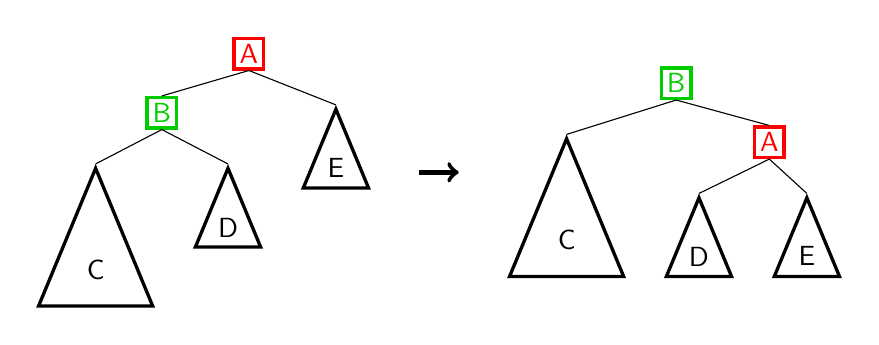
\begin{tikzpicture}
  [every tree node/.style = {
    align=center, inner sep=2pt, text centered, font=\sffamily, 
    rectangle, black, draw=black, very thick},
   every leaf node/.style = {draw=none},
   n/.style = {draw=none},
   level distance=0.75cm, sibling distance=0.5cm,
   subtree/.style = 
     {isosceles triangle, shape border rotate=90, anchor=north, yshift=1mm, inner sep=0cm}
  ]
  \node(before) {
    \Tree [.\node[color=red]{A}; 
      [.\node[color=green!80!black]{B}; 
        [.\node[subtree, minimum height=1.75cm]{C}; ]
        [.\node[subtree, minimum height=1cm]{D}; ]        
      ]
      [.\node[subtree, minimum height=1cm]{E}; ] ]
  }; 
  \node(after) [at={($(before.east) + (1.5cm,0)$)}, anchor=west] {
    \Tree [.\node[color=green!80!black]{B}; 
      [.\node[subtree, minimum height=1.75cm]{C}; ] 
      [.\node[color=red]{A}; 
        [.\node[subtree, minimum height=1cm]{D}; ] 
        [.\node[subtree, minimum height=1cm]{E}; ] ] ]
  };
  \draw[->, ultra thick] ($(before.east) + (0.5cm,0)$) -- ($(after.west) - (0.5,0)$); 
\end{tikzpicture}
\end{document}